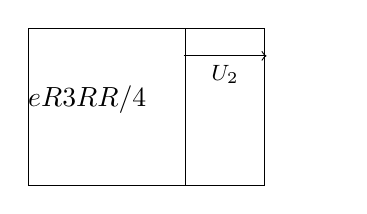
\begin{tikzpicture}[font=\footnotesize]
	\draw (0,-1)rectangle(3,1);
	\draw (2,-1)--++(0,2);
	\pileL{}{$e$};
	\resistanceV{shift={(2,0)}}{$R$};
	\resistanceV{shift={(3,0)}}{$3R$};
	\resistanceH{shift={(1,1)}}{$R/4$};
	\draw[shift={(3,0)},->](10pt,-15pt)--++(0,30pt)node[midway,right]{$U_1$};
	\draw[shift={(1,1)},->](-15pt,-10pt)--++(30pt,0)node[midway,below]{$U_2$};
\end{tikzpicture}